\documentclass[a4paper, 11pt]{article}
\usepackage{fullpage} 
\usepackage[margin=1.25cm]{geometry}
\usepackage{graphicx}
\usepackage{enumitem}
\usepackage{fancyhdr}
\usepackage{multicol}
\usepackage{xhfill}
\usepackage{changepage}

\title{Final Hack Report}\author{Andy Wong\\Glen Chou\\Lydia Lee}\date{Due: May 5, 2015}
\setlength{\headsep}{1cm}

\begin{document}
\pagestyle{fancy}
\fancyhf{}
\lhead{Final Hack Report}
\rhead{A. Wong, G. Chou, L. Lee}
\chead{Team Turret}
\maketitle
\tableofcontents

\newpage
\section{Features}
YOU CAN INSERT AN ABSTRACT OR BRIEF GENERAL DESCRIPTION HERE.
	\subsection{Rotating Platform}
		1 motor is controlled with proportional and integral controls (PID).  The joystick allows user control over the turret's rotation.
	\subsection{Rubber Band Gun}
\newpage
\section{Schematics}
	\subsection{Table Motor}
		\begin{center}
			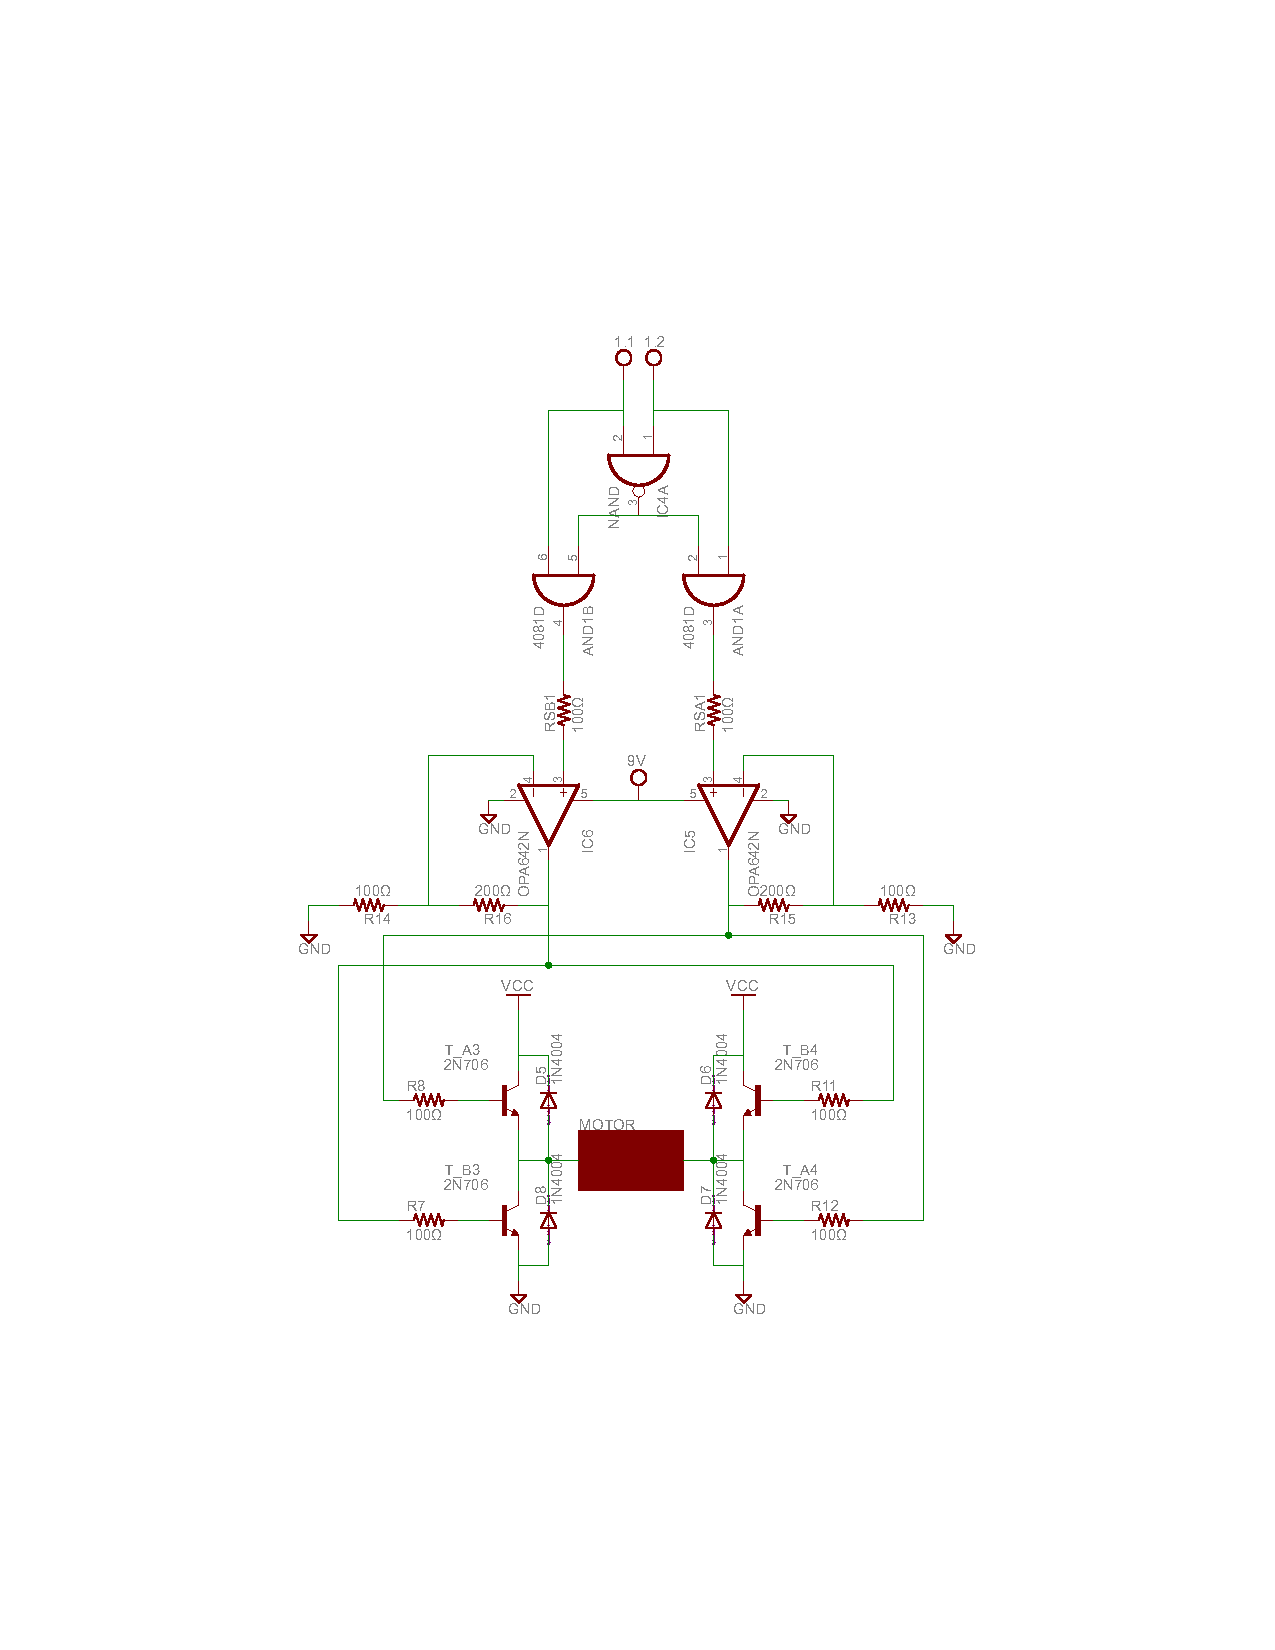
\includegraphics{bidirectional-motor-driver}
		\end{center}
	\subsection{Firing Mechanism}
		\begin{center}
%			\includegraphics{}
		\end{center}
	\subsection{Joystick}
		\begin{center}
%			\includegraphics{}
		\end{center}
\section{Code}
% A brief description of extra features (4 lines per feature)
% b. Schematic diagram of the additional analog circuitry
% c. Your MSP430 code with small comment lines explaining the function of each code block.

\end{document}